\documentclass{article}
\usepackage[utf8x]{inputenc}
\usepackage{ucs}
\usepackage{amsmath} 
\usepackage{amsfonts}
\usepackage{upgreek}
\usepackage[english,russian]{babel}
\usepackage{graphicx}
\usepackage{float}
\usepackage{textcomp}
\usepackage{hyperref}
\usepackage{geometry}
  \geometry{left=2cm}
  \geometry{right=1.5cm}
  \geometry{top=1cm}
  \geometry{bottom=2cm}
\usepackage{tikz}
\usepackage{ccaption}
\usepackage{multicol}
%\setlength{\columnsep}{1.5cm}
%\setlength{\columnseprule}{0.2pt}
\usepackage{listings}

\begin{document}
\pagenumbering{gobble}

\lstset{
  language=C,                % choose the language of the code
  basicstyle=\linespread{1.1}\ttfamily,
  columns=fixed,
  fontadjust=true,
  basewidth=0.5em,
  keywordstyle=\color{blue}\bfseries,
  commentstyle=\color{gray},
  stringstyle=\ttfamily\color{orange!50!black},
  showstringspaces=false,
  %numbers=false,                   % where to put the line-numbers
  numbersep=5pt,
  numberstyle=\tiny\color{black},
  numberfirstline=true,
  stepnumber=1,                   % the step between two line-numbers.        
  numbersep=10pt,                  % how far the line-numbers are from the code
  backgroundcolor=\color{white},  % choose the background color. You must add \usepackage{color}
  showstringspaces=false,         % underline spaces within strings
  captionpos=b,                   % sets the caption-position to bottom
  breaklines=true,                % sets automatic line breaking
  breakatwhitespace=true,         % sets if automatic breaks should only happen at whitespace
  xleftmargin=.2in,
  extendedchars=\true,
  keepspaces = true,
}
\lstset{literate=%
   *{0}{{{\color{red!20!violet}0}}}1
    {1}{{{\color{red!20!violet}1}}}1
    {2}{{{\color{red!20!violet}2}}}1
    {3}{{{\color{red!20!violet}3}}}1
    {4}{{{\color{red!20!violet}4}}}1
    {5}{{{\color{red!20!violet}5}}}1
    {6}{{{\color{red!20!violet}6}}}1
    {7}{{{\color{red!20!violet}7}}}1
    {8}{{{\color{red!20!violet}8}}}1
    {9}{{{\color{red!20!violet}9}}}1
}


\title{Семинар \#11: Связный список.\vspace{-5ex}}\date{}\maketitle
Создадим структуру \texttt{Node}, которая будет содержать:
\begin{itemize}
\item \textbf{Данные}: одно или несколько полей каких-угодно типов. В данном случае это 1 переменная \texttt{value}.
\item \textbf{Связь}: указатель \texttt{next} на структуру того же типа \texttt{Node}.
\end{itemize}
\begin{center}
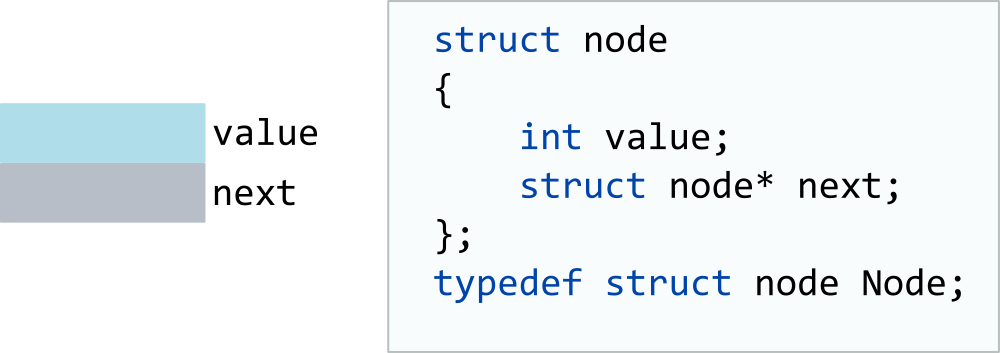
\includegraphics[scale=0.8]{../images/codelist/codelist1.png}
\end{center}

Используя такую структуру, можно создать Связный список:
\begin{center}
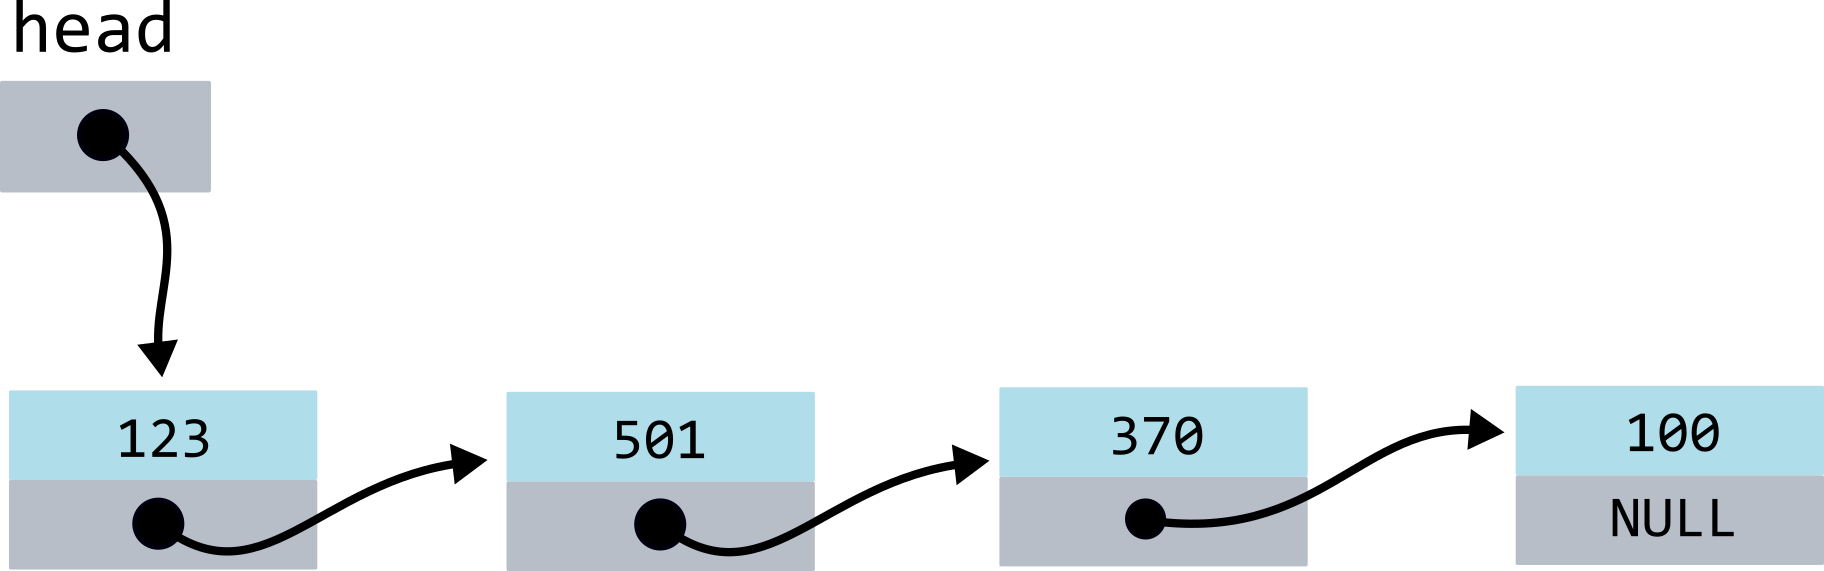
\includegraphics[scale=0.8]{../images/codelist/codelist_only.png}
\end{center}
\textit{Примечание}: \texttt{NULL} - это просто константа равная 0. Её используют вместо нуля для указателей, чтобы различать числовые переменные и указатели.

\subsubsection*{Вычислительные сложности операций со списком:}
\begin{center}
\begin{tabular}{ c c c }
 Операция & Массив & Односвязный список \\ 
 \hline
 Доступ по номеру & $O(1)$ & $O(N)$  \\
 Поиск & $O(N)$ & $O(N)$  \\    
 Вставка в начало & $O(N)$ & $O(1)$  \\
 Вставка в конец & $O(1)$ & $O(N)$  \\
 \begin{tabular}{@{}c@{}}Вставка в конец если известен \\ указатель на последний элемент\end{tabular} & $O(1)$ & $O(1)$  \\
 Вставка в середину & $O(N)$ & $O(N)$  \\
 \begin{tabular}{@{}c@{}}Вставка в середину если известен \\ указатель на предыдущий элемент\end{tabular} & $O(N)$ & $O(1)$  \\  
\end{tabular}
\end{center}

Чему равны вычислительные сложности следующих операций:
\begin{itemize}
\item Нахождение размера списка. Что можно сделать, чтобы нахождение размера выполнялось быстрее?
\item Удаление элемента из начала списка.
\item Удаление элемента из конца списка. Что нужно знать, чтобы эта операция выполнялась быстрее?
\item Удаление элемента из середины списка. Что нужно знать, чтобы эта операция выполнялась быстрее?
\end{itemize}

\newpage
\subsection*{Задачи. Напишите следующие функции для работы со связным списком:}
Начальный код в файле \texttt{list.c}.
\begin{enumerate}
\item \texttt{Node* list\_create()} -- инициализирует список (создаёт и возвращает список нулевого размера). Эта функция просто возвращает \texttt{NULL}. Зачем нужна такая простая функция? Она нужна для согласованности с реализациями других структур данных. Например, при реализации хеш-таблицы у нас будет более сложная функция \texttt{hashtable\_create}, которая будет создавать хеш-таблицу.
\item \texttt{void list\_add\_first(Node** p\_head, int x)} -- добавляет элемент x в начало списка. Чтобы добавить элемент, нужно для начала выделить необходимое количество памяти под этот элемент, затем задать поля нового элемента таким образом, чтобы он указывал на начало списка. В конце нужно поменять значение указателя на начало списка. Обратите внимание, что так как нужно изменить значение указателя, то в эту функцию нужно передавать указатель на указатель.
\item \texttt{void list\_add\_last(Node** p\_head, int x)} -- добавляет элемент x в конец списка. (решение этой задачи есть в файле \texttt{list.c}).
\item \texttt{int list\_remove\_first(Node** p\_head)} -- удаляет элемент из начала списка и возвращает его значение. Не забудьте изменить \texttt{*p\_head}.
\item \texttt{int list\_remove\_last(Node** p\_head)} -- удаляет элемент из конца списка и возвращает его значение. 
\item \texttt{void list\_print(const Node* head)} -- распечатывает все элементы списка.
\item \texttt{int list\_size(const Node* head)} -- возвращает количество элементов списка.
\item \texttt{int list\_destroy(Node* head)} -- освобождает всю память, выделенную под список. Так как память выделялась под каждый элемент отдельно, то освобождать нужно также каждый элемент по отдельности.

\item \texttt{void list\_reverse(Node** p\_head)} -- переворачивает связный список. Первый элемент становится последним, а последний первым. В данной задаче вам не нужно перемещать элементы \texttt{value} или сами структуры. Нужно просто изменить указатели.

\item \texttt{void list\_concatenate(Node** p\_head1, Node** p\_head2)}, которая добавляет второй связный список в конец первого.

\item Реализовать абстрактный тип данных стек(Stack) на основе связного списка. 

\item Создайте связный список размера 10. Последний элемент должен ссылаться на 5-й. Что будет, если попробовать напечатать такой список?

\item Написать функцию \texttt{int list\_is\_loop(Node* head)}, которая проверяет, если в связном списке цикл.

\item Написать функцию \texttt{int list\_fix\_loop(Node* head)}, которая проверяет, если в связном списке цикл. И если цикл есть, то она размыкает его.
\end{enumerate}
\begin{center}
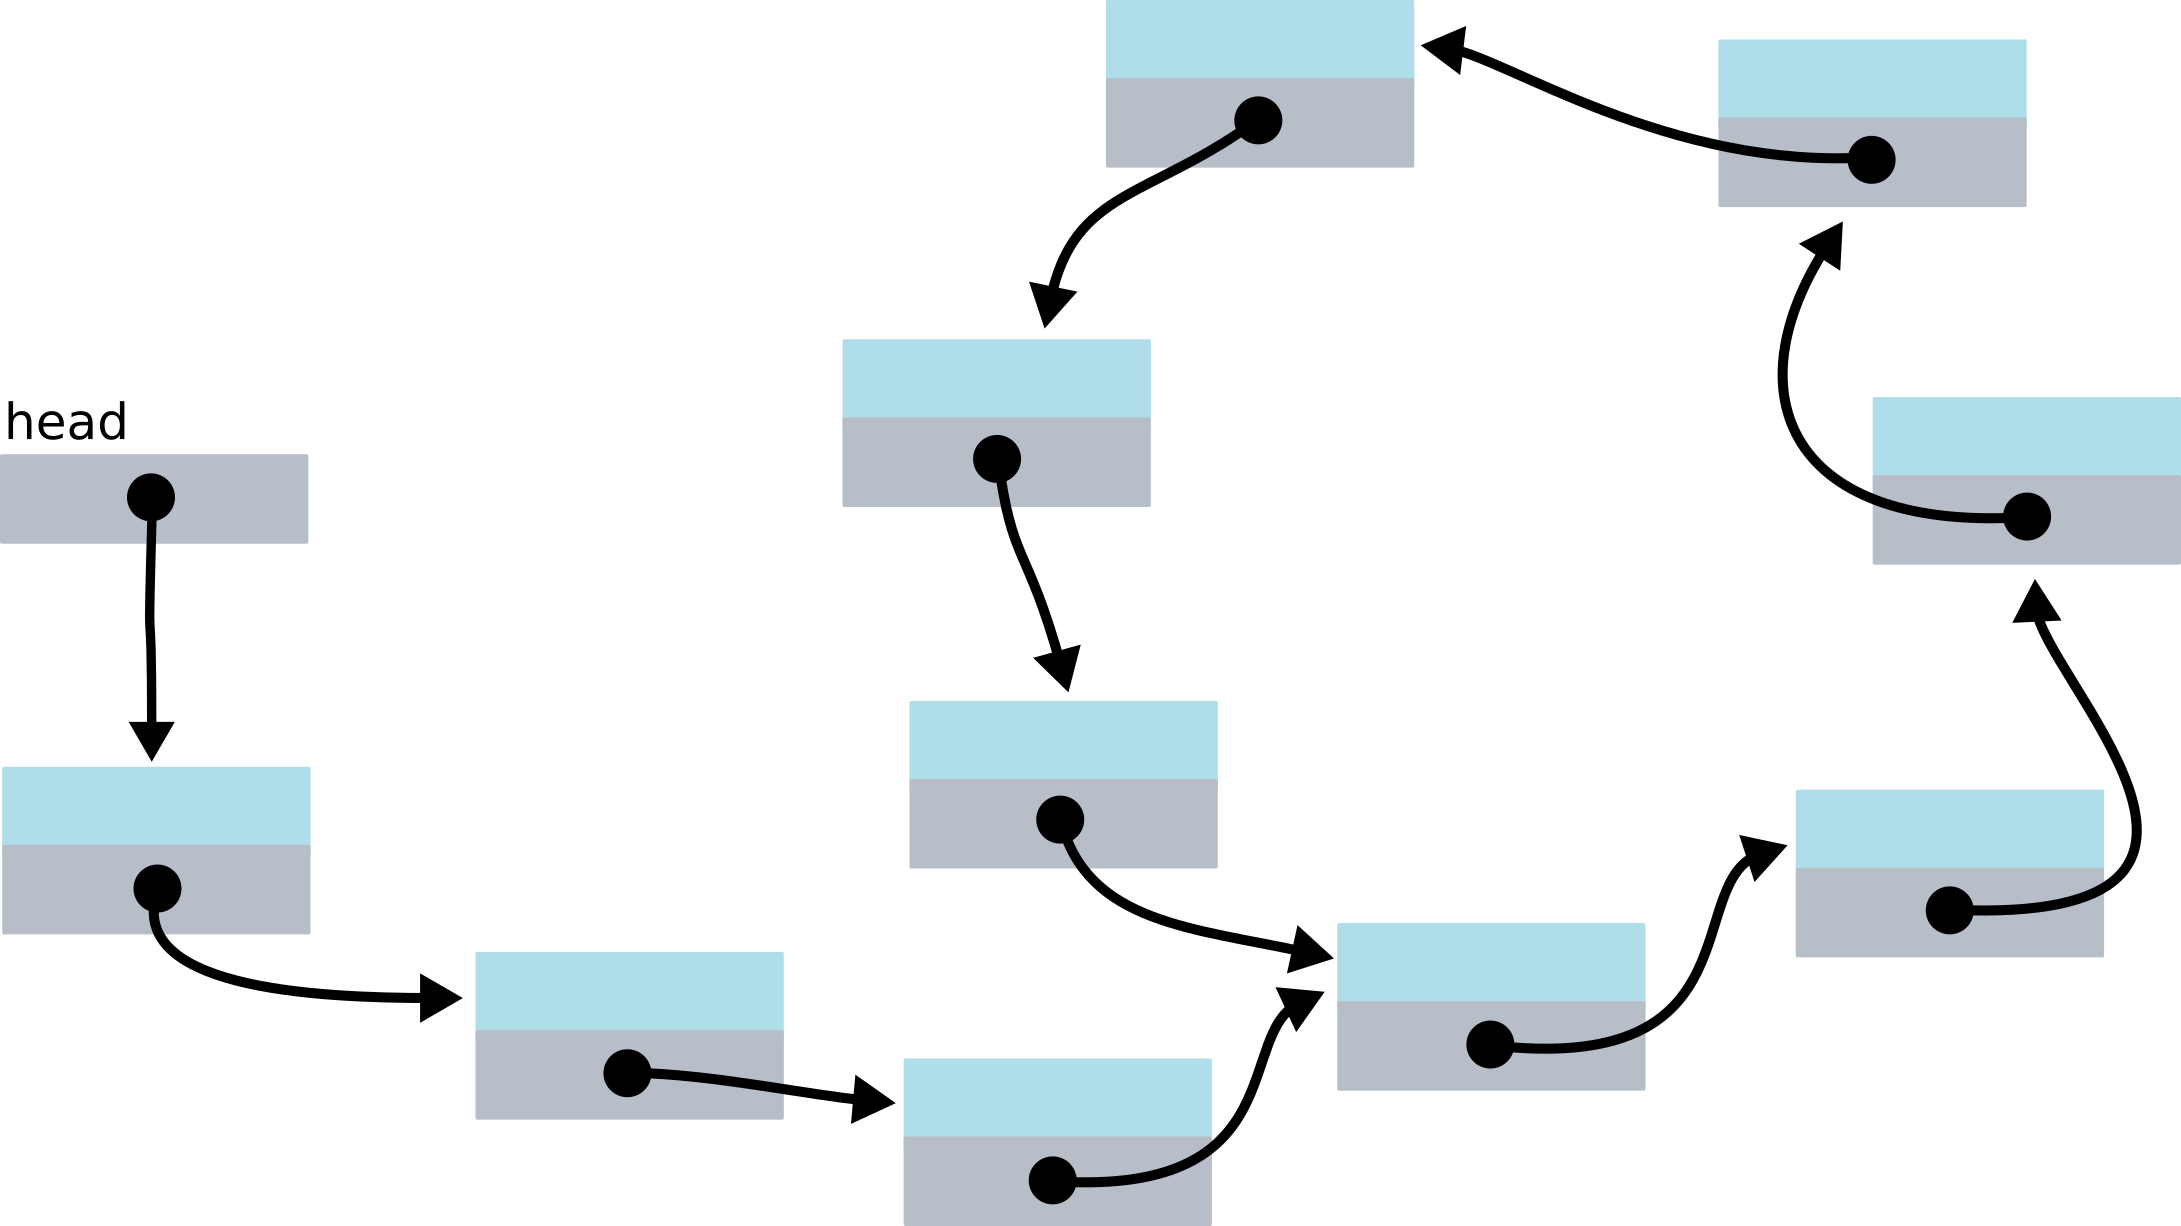
\includegraphics[scale=0.77]{../images/list_loop_2.png}
\end{center}






\end{document}